%%%%%%%%%%%%%%%%%%%%%%%%%%%%%%%%%%%%%%%%%%%%%%%%%%%%%%%%%%%%%%%%%%%%%%%%%%%%%%%
%
% Data tests
% 
%%%%%%%%%%%%%%%%%%%%%%%%%%%%%%%%%%%%%%%%%%%%%%%%%%%%%%%%%%%%%%%%%%%%%%%%%%%%%%%
\chapter{Data tests}
\label{cha6}

In order to examine our application and to prove the efficiency of it, we want to run the application on several invoice documents. Using 300 invoice documents that each contain different company names, positions, values and layouts we have come to a conclusion to our work.
Before we present our results, we want to explain what has been measured and how we define \"accurate\".
There are multiple fields in an invoice document that are important for processing. To be able to provide the possibility to convert the document into an electronic invoice format we need to provide at least the following:
\begin{itemize}
\itemsep -1em 
	\item The invoice number
	\item The issue date
	\item The debitor (or as called in the ZugFerd specification: buyer)
	\item The creditor (or as called in the ZugFerd specification: seller)
	\item Line Total
	\item Charge Total
	\item Allowance Total
	\item Tax Basis Total
	\item Tax Total
	\item Grand Total
	\item The delivery date
\end{itemize}

We will calculate accuracy by counting all fields that have been found and are correct. This means, every correct field will lead to an increased accuracy of $\frac{1}{11}$ in total. A processed document that leads to 11 correctly found fields will result to 100\% accuracy. 

As this application learns over time, we expect the accuracy to increase over time. Hence we will not only sum up the accuracy by using all results, but also show the accuracy evolution over time.

Table \ref{accuracyTable} shows the resulting accuracy of the processed invoice documents: 
\begin{figure}[ht!]
\centering
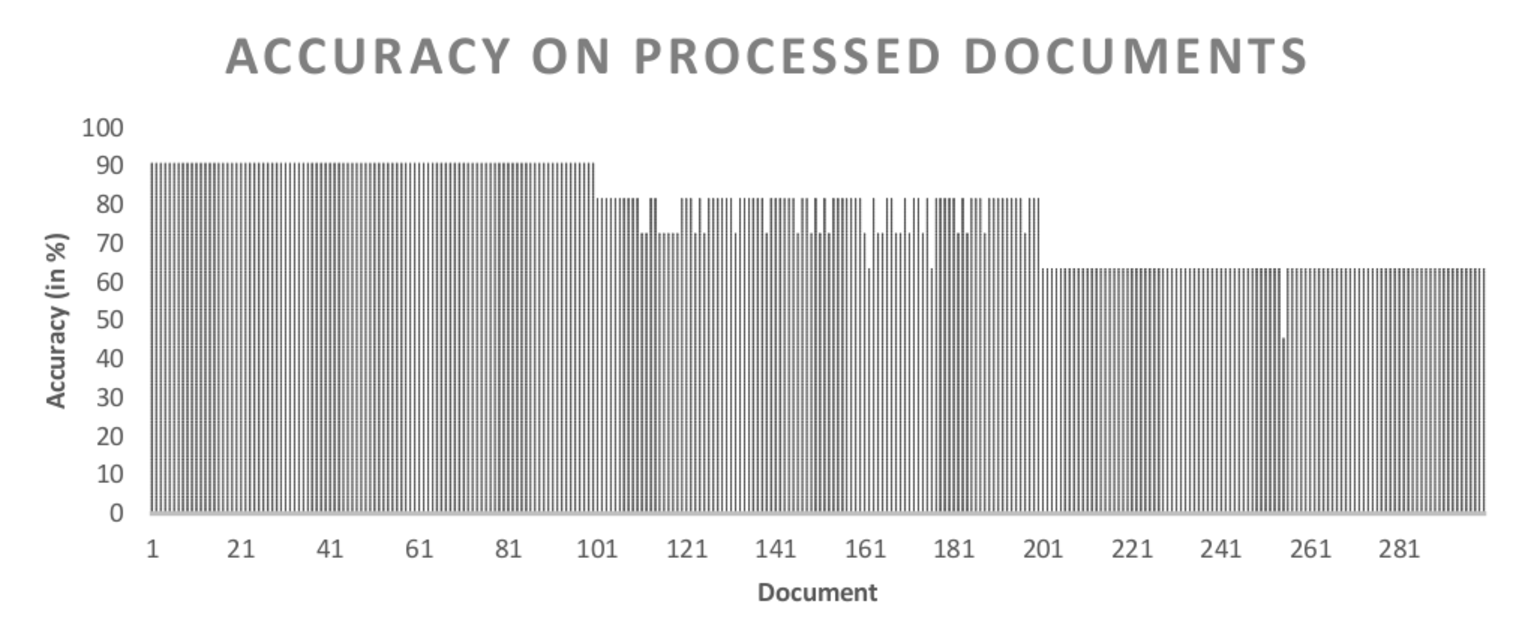
\includegraphics[width=\textwidth]{Images/Accuracy/accuracyTable.pdf}
\caption{Resulting accuracy of the application \label{accuracyTable}}
\end{figure}

There are especially two things that can be seen clearly in this table. First, the accuracy drops between the 100st and 200st document. This can be explained due to the fact that at this point another layout has been used. This also shows that the application is still dependent by the layout of the invoice document.

Secondly, the accuracy of the document processing is equal for each template (except some distortions). This indicates that our algorithm works data independently and its performance is mainly controlled by the document layout.

Eventually, we want to talk about the accuracy presented here. In all of the given invoices there was always one information missing: The seller. This can be explained because of a missing learning step. In a normal case, the application would learn about a creditor the first time a document is processed. The next time, the application would be able to retrieve information of that creditor. Due to our automated testing approach, this step is missing. Hence there are missing information.
We took 10 documents of each layout and processed them manually in order to prove that explanation. Figure (TODO: FIGURE) shows the accuracy compared to the previous one. Due to the information given to the application the new accuracy is higher than before.

This leads to the final presentation of the overall accuracy of the algorithm. Without the learning of a creditor, the application is able to process invoice documents with an accuracy of 77,81\%.